\section{Introduction}

Variant pathogenicity prediction prioritizes variants for expert review, but biological evidence, labels, and partitions are interdependent. Agreement with ClinVar assertions \cite{landrum2018clinvar} is distinct from applying ACMG/AMP criteria to an individual case \cite{richards2015acmg}. A benchmark score therefore needs an explicit evidence boundary and evaluation population.

dbNSFP distributes existing predictor scores \cite{liu2020dbnsfp}, potentially importing their training history. Separately, variants from the same gene can cross a random split despite coordinate deduplication. Variant/protein overlap creates circularity \cite{grimm2015circularity}. Excluding scores and separating genes address distinct dependencies; neither guarantees useful performance within each consequence.

MX-Audit evaluates the local MAGPIE-X LightGBM pipeline, not the released MAGPIE model or an endorsed extension. We stratify errors and decompose ranking pairs, supported by ablations, simple baselines, exact-row comparators, and repeated partition controls. The question is what pooled ranking conceals, not whether a new architecture wins a benchmark.

\emph{Low-circularity} denotes the explicit feature boundary, not freedom from ascertainment, annotation dependence, or biological relatedness.

\begin{figure*}[t]
\centering
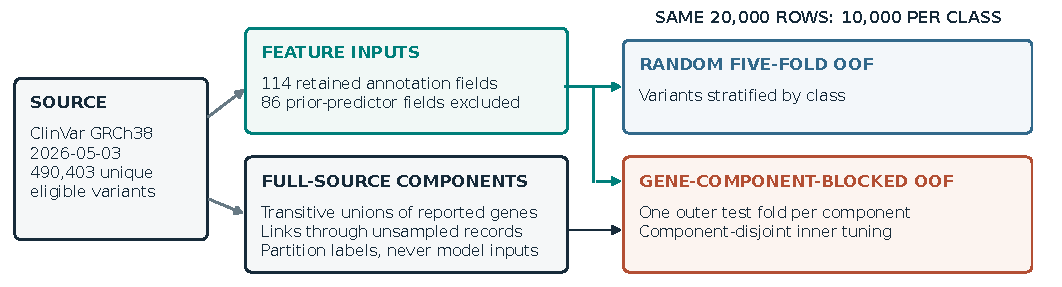
\includegraphics[width=\textwidth]{figures/experimental_design.pdf}
\caption{Full-source gene unions precede balanced sampling, preserving links through unsampled records. Each sampled row receives random and blocked OOF predictions. Inner tuning uses outer training rows only, with disjoint components in the blocked arm. Gene identifiers define partitions, never inputs.}
\label{fig:design}
\end{figure*}
